\documentclass[11pt]{article}
\usepackage[
top    = 2.50cm,% presumably you don't want it to be 0pt as well?
bottom = 2.50cm,
left   = 2cm,
right  = 2cm,
marginparsep = 0pt,
marginparwidth=0pt,
]{geometry}

\usepackage{amssymb}
\usepackage{fancyhdr}
\usepackage[most]{tcolorbox}
\usepackage{siunitx}
\usetikzlibrary{calc,patterns,angles,quotes}
\usepackage{amsmath}
\usepackage{tikz, tikz-3dplot}
\usepackage{caption}
\usepackage{pgfplots}
\usepackage{multicol}
\pagestyle{fancy}
\fancyhead[l]{Waves - Abridged edition}
\fancyhead[r]{Giorgio Grigolo {\textcopyright}}
\newcommand\textcenter[1]{
	\begin{center}
		#1
	\end{center}
}
\begin{document}
	\section{Simmple Harmonic Motion: }
	\subsection{Definition: }
\begin{center}
		The type of oscillatory motion in which the acceleration of the oscillating body is proportinal  to the body's displacement from the equilibrium position and always acts towards the equilibrium position.
\end{center}
	\subsection{Graph: }
	\begin{center}
		{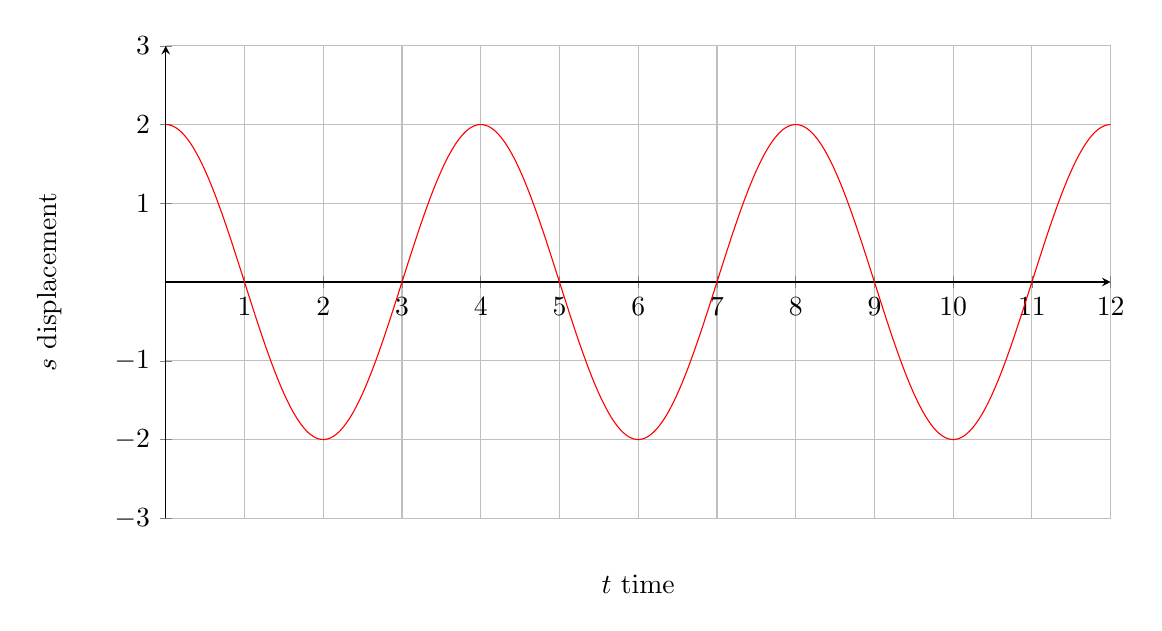
\begin{tikzpicture}[scale=1]
				\begin{axis}[
					x=1cm,y=1cm,
					axis lines=middle,
					ymajorgrids=true,
					xmajorgrids=true,
					xmin=0,
					xmax=12,
					ymin=-3,
					x label style={at={(axis description cs:0.5,-0.1)},anchor=north},
					y label style={at={(axis description cs:-0.1,0.5)},rotate=90,anchor=south},
					xlabel=$t$ time,
					ylabel=$s$ displacement,
					ymax=3,
					xtick={0,1,...,12},
					ytick={-3,-2,...,3},]
					\addplot[color=red, domain=0:12,samples=1000]{2*sin(90*(x+1))};
				\end{axis}
			\end{tikzpicture}
			\captionof*{figure}{}}
	\end{center}
	\subsection{Diagram: }
	\begin{center}
		\begin{tikzpicture}[scale=1.6]
			% save length of g-vector and theta to macros
			\pgfmathsetmacro{\Gvec}{1.5}
			\pgfmathsetmacro{\myAngle}{45}
			% calculate lengths of vector components
			\pgfmathsetmacro{\Gcos}{\Gvec*cos(\myAngle)}
			\pgfmathsetmacro{\Gsin}{\Gvec*sin(\myAngle)}
			
			\coordinate (centro) at (0,0);
			\draw[dashed,gray,-] (centro) -- ++ (0,-3.5) node (mary) [black,below]{$ $};
			\draw[thick] (centro) -- ++(270+\myAngle:3) coordinate (bob);
			\pic [draw, ->, "$\theta$", angle eccentricity=1.5] {angle = mary--centro--bob};
			\draw [blue,-stealth] (bob) -- ($(bob)!\Gcos cm!(centro)$);
			\draw [-stealth] (bob) -- ($(bob)!-\Gcos cm!(centro)$)
			coordinate (gcos)
			node[midway,above right] {$mg\cos\theta$};
			\draw [-stealth] (bob) -- ($(bob)!\Gsin cm!90:(centro)$)
			coordinate (gsin)
			node[midway,above left] {$mg\sin\theta$};
			\draw [-stealth] (bob) -- ++(0,-\Gvec)
			coordinate (g)
			node[near end,left] {$mg$};
			\pic [draw, ->, "$\theta$", angle eccentricity=1.5] {angle = g--bob--gcos};
			\filldraw [fill=black!40,draw=black] (bob) circle[radius=0.1];
		\end{tikzpicture}
	\end{center}
	\subsection{Equation: }
	\begin{equation}
		a = -\frac{4\pi^2}{T^2} \times x\tag{\si{\meter\per\second\squared}}
	\end{equation}

\begin{center}
	Where $T$ is the \textbf{periodic time} (\si{\second}).
\end{center}
	
	\section{Phase difference: }
\subsection{\textcolor{blue}{$\frac{T}{4}$}, \textcolor{green}{$\frac{T}{2}$} phase difference: }
	\begin{center}
		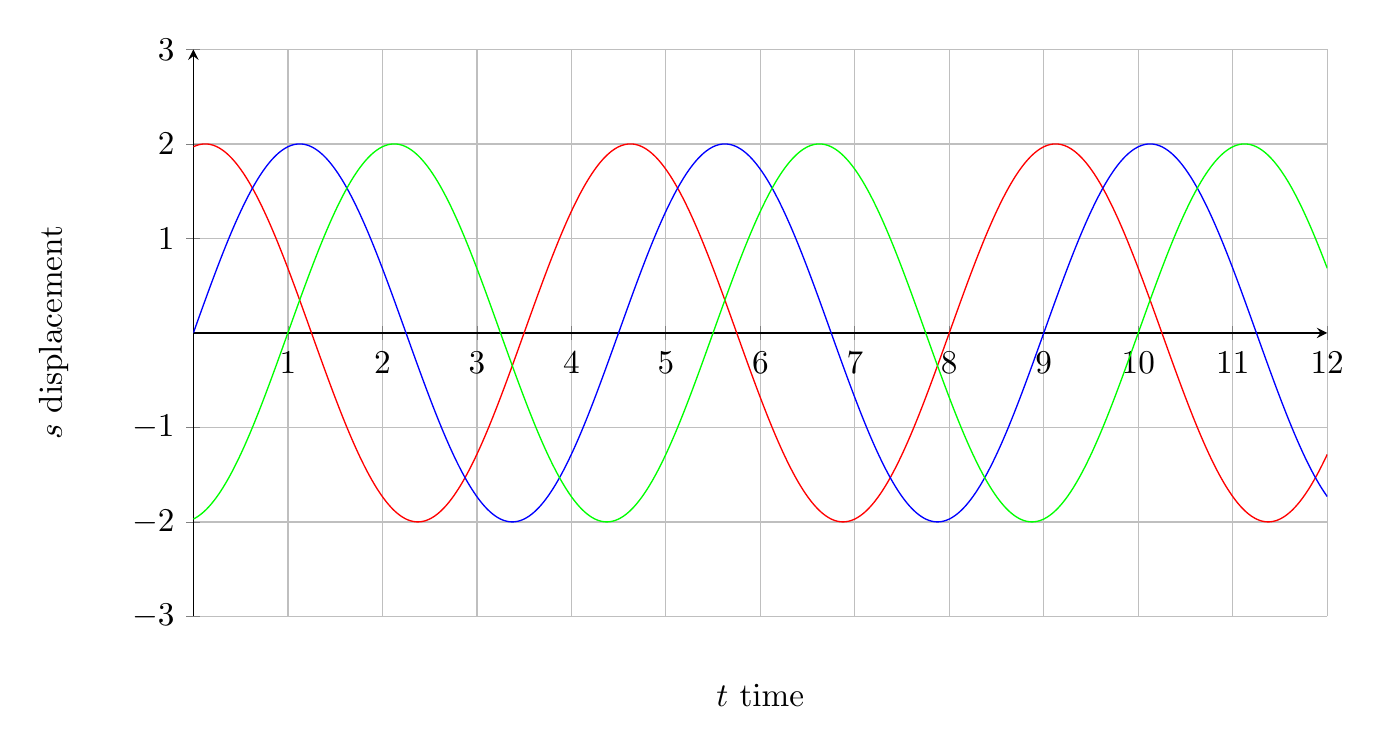
\begin{tikzpicture}[scale=1.2]
				\begin{axis}[
					x=1cm,y=1cm,
					axis lines=middle,
					ymajorgrids=true,
					xmajorgrids=true,
					xmin=0,
					xmax=12,
					ymin=-3,
					x label style={at={(axis description cs:0.5,-0.1)},anchor=north},
					y label style={at={(axis description cs:-0.1,0.5)},rotate=90,anchor=south},
					xlabel=$t$ time,
					ylabel=$s$ displacement,
					ymax=3,
					xtick={0,1,...,12},
					ytick={-3,-2,...,3},]
					\addplot[color=red, domain=0:12,samples=1000]{2*sin(80*(x+1))};
					\addplot[color=blue, domain=0:12,samples=1000]{2*sin(80*(x))};
					\addplot[color=green, domain=0:12,samples=1000]{2*sin(80*(x-1))};
				\end{axis}
			\end{tikzpicture}
	\end{center}

\subsection{Full representation of SHM: }
\begin{center}
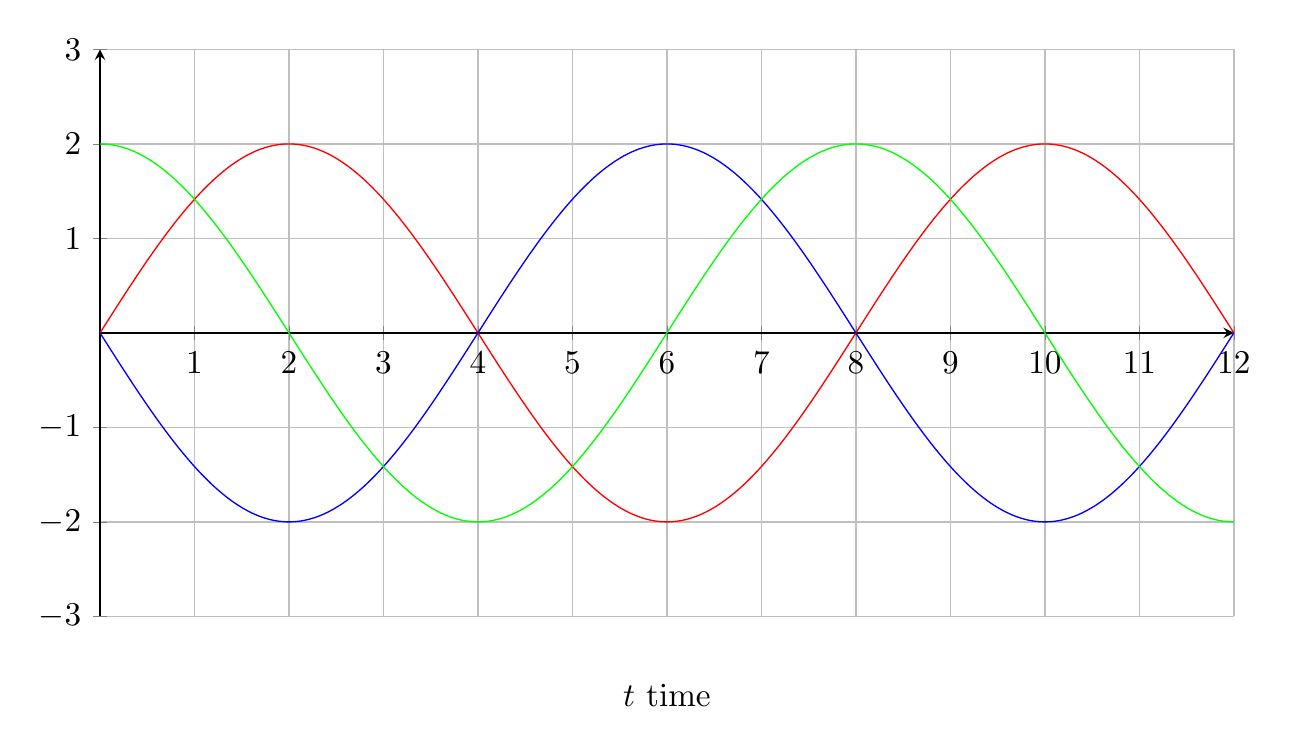
\begin{tikzpicture}[scale=1.2]
		\begin{axis}[
			x=1cm,y=1cm,
			axis lines=middle,
			ymajorgrids=true,
			xmajorgrids=true,
			xmin=0,
			xmax=12,
			ymin=-3,
			x label style={at={(axis description cs:0.5,-0.1)},anchor=north},
			y label style={at={(axis description cs:-0.1,0.5)},rotate=90,anchor=south},
			xlabel=$t$ time,
			ymax=3,
			xtick={0,1,...,12},
			ytick={-3,-2,...,3},]
			\addplot[color=red, domain=0:12,samples=1000]{2*sin(45*(x))};
			\addplot[color=blue, domain=0:12,samples=1000]{2*sin(45*(-x))};
			\addplot[color=green, domain=0:12,samples=1000]{2*sin(45*(x+2};
		\end{axis}
	\end{tikzpicture}
	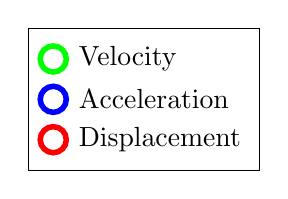
\begin{tikzpicture}[
		blacknode/.style={shape=circle, draw=black, line width=2},
		bluenode/.style={shape=circle, draw=blue, line width=2},
		greennode/.style={shape=circle, draw=green, line width=2},
		rednode/.style={shape=circle, draw=red, line width=2}
		]
		\matrix [draw,below left] at (0,0) {
			\node [greennode,label=right:Velocity] {}; \\
			\node [bluenode,label=right:Acceleration] {}; \\
			\node [rednode,label=right:Displacement] {}; \\
		};
	\end{tikzpicture}
\end{center}

\section{$n$\textsuperscript{th} harmonic}

\begin{equation}
	f_n = \frac{n }{2l}\sqrt{\frac{T}{\mu}}
\end{equation}

\begin{center}
	Where $l$ is the \textbf{length} (\si\meter) of the given string, $T$ the \textbf{tension} (\si\newton) present through it and $\mu$ its \textbf{linear mass density} (\si{\kilogram\per\meter}).
\end{center}
\section{Young's Double Slit Experiment}

\begin{center}
	 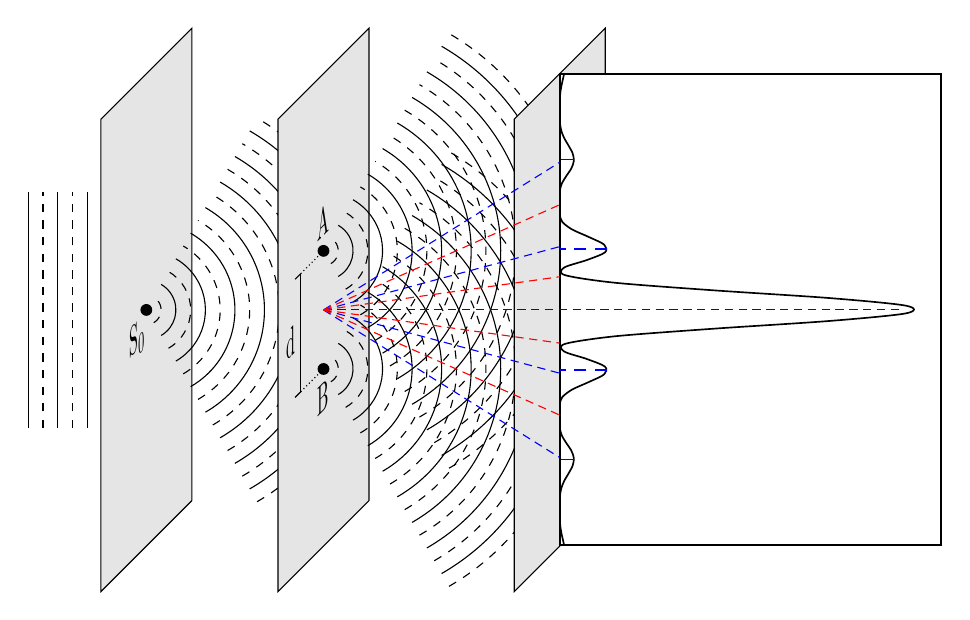
\begin{tikzpicture}[scale=1.5,every node/.append style={transform shape}]
	 	\foreach \x in {-0.5,-0.25,0} {
	 		\draw (\x,-1) -- (\x,1);
	 	}
	 	\foreach \x in {-0.375,-0.125,-0.125} {
	 		\draw[dashed] (\x,-1) -- (\x,1);
	 	}
	 	\draw[fill=black!10] (0.5,-2,-1) -- (0.5,-2,1) -- (0.5,2,1) -- (0.5,2,-1) -- (0.5,-2,-1);
	 	\fill (0.5,0,0) circle (0.05);
	 	\foreach \r in {0.25,0.5,...,1.75} {
	 		\draw (0.5,0) ++(-60:\r) arc (-60:60:\r);
	 	}
	 	\foreach \r in {0.125,0.375,...,1.875} {
	 		\draw[dashed] (0.5,0) ++(-60:\r) arc (-60:60:\r);
	 	}
	 	\draw[fill=black!10] (2,-2,-1) -- (2,-2,1) -- (2,2,1) -- (2,2,-1) -- (2,-2,-1);
	 	\fill (2,0.5) circle (0.05) (2,-0.5) circle (0.05);
	 	\foreach \r in {0.25,0.5,...,2} {
	 		\draw (2,0.5) ++(-60:\r) arc (-60:60:\r);
	 		\draw (2,-0.5) ++(-60:\r) arc (-60:60:\r);
	 	}
	 	\foreach \r in {0.125,0.375,...,2.125} {
	 		\draw[dashed] (2,0.5) ++(-60:\r) arc (-60:60:\r);
	 		\draw[dashed] (2,-0.5) ++(-60:\r) arc (-60:60:\r);
	 	}
	 	\draw (2,0.5,0.625) -- (2,0.5,0.5);
	 	\draw (2,-0.5,0.625) -- (2,-0.5,0.5);
	 	\draw (2,0.5,0.5) -- (2,-0.5,0.5);
	 	\draw[densely dotted] (2,0.5,0.5) -- (2,0.5,0);
	 	\draw[densely dotted] (2,-0.5,0.5) -- (2,-0.5,0);
	 	\draw[fill=black!10] (4,-2,-1) -- (4,-2,1) -- (4,2,1) -- (4,2,-1) -- (4,-2,-1);
	 	%       LABELLING
	 	\begin{scope}[canvas is yz plane at x=2,rotate=-90]
	 		\node[above] at (0,0.5) {A};
	 		\node[below] at (0,-0.5) {B};
	 		\node[left] at (-0.5,0) {d};
	 	\end{scope}
	 	\begin{scope}[canvas is yz plane at x=0.5,rotate=-90]
	 		\node[below left=-0.1cm] at (0,0) {S${}_0$};
	 	\end{scope}
	 	\begin{scope}[xshift=4cm,yshift=2cm,rotate=-90,canvas is xy plane at z=0]
	 		\fill[white] (0,0) rectangle (4,1);
	 		\begin{axis}[
	 			width=5.575cm,
	 			xmin=-0.62,
	 			xmax=0.62,
	 			ymin=0,
	 			ticks=none
	 			]
	 			\addplot [samples=500,black,smooth
	 			]
	 			{(cos(deg(5*pi*sin(deg(x)))))^(2)*((sin(deg(4*pi*sin(deg(x)))))/(4*pi*sin(deg(x))))^(2)};
	 			\draw[thin, densely dashed,blue] (axis cs:0.1593,0.1327) -- (axis cs:0.1593,0);
	 			\draw[thin, densely dashed,blue] (axis cs:-0.1593,0.1327) -- (axis cs:-0.1593,0);
	 			\draw[thin, densely dashed,blue] (axis cs:0.3941,0.03938) -- (axis cs:0.3941,0);
	 			\draw[thin, densely dashed,blue] (axis cs:-0.3941,0.03938) -- (axis cs:-0.3941,0);
	 		\end{axis}
	 	\end{scope}
	 	\draw[thin,densely dashed,blue] (2,0) -- (6.9,0);
	 	\begin{scope}
	 		\clip (2,-2) rectangle (4,2);
	 		\draw[thin,densely dashed,blue] (2,0) --    +(15:4);
	 		\draw[thin,densely dashed,blue] (2,0) --    +(-15:4);
	 		\draw[thin,densely dashed,blue] (2,0) --    +(32:4);
	 		\draw[thin,densely dashed,blue] (2,0) --    +(-32:4);
	 		\draw[thin,densely dashed,red] (2,0) --     +(8:4);
	 		\draw[thin,densely dashed,red] (2,0) --     +(-8:4);
	 		\draw[thin,densely dashed,red] (2,0) --     +(24:4);    
	 		\draw[thin,densely dashed,red] (2,0) --     +(-24:4);               
	 	\end{scope}
	 \end{tikzpicture}\\
The observable pattern achieved in this experiment can be seen above. It consists of alternate dark and bright bands. The centreal band, the one equidistant from both slits is always bright ($AO - BO = 0\lambda$)
\begin{multicols}{2}
	destructive interference $\implies$ dark\\
	constructive interference $\implies$ bright
\end{multicols}
\end{center}
\subsection{Path difference}
\begin{multicols}{2}
	\begin{center}
		\textbf{\underline{Bright band}}\\
		~\\
		$n\lambda,\, n \in \mathbb{N}$
	\end{center}
	\begin{center}
	\textbf{\underline{Dark band}}\\
	~\\
	$n\frac12\lambda,\, n \in \mathbb{N}$
\end{center}
\end{multicols}
\subsection{Bright slit interval distance: }
\begin{equation}
	y=\frac{D\lambda}{d}\tag{\si{\meter}}
\end{equation}
\begin{center}
	Where $D$ is the \textbf{distance} (\si{\meter}) between the slits and the screen, $d$ is the \textbf{seperation} ({\si{\meter}}) between the two slits and $\lambda$ the \textbf{wavelength} (\si{\meter}) of the wave at the source.
\end{center}
\end{document}